
\section{2D Solver}
\subsection{1D Conservation Laws}
We expect the following quantities to be conserved: mass h, momentum or mass velocity, $hu$ and $hv$, and
energy 0.5($hv^2$+$gh^2$). Potential vorticity is only looked at in the 2D solver. Invesigation of conservation of momentum in solver.
 Is the momentum conserved, what explanation do we have?

The spatial domain for the 2D solver is $\Omega [1\;\;1]$ To go about solving the system in 2D there are many options,
we compare two schemes. Lax-Wendfoff, and a two step version of Richtmeyer proposed. \newline
\newline

\subsection{Dimensional Splitting (Lax Wendroff)}

Using the 1D equations of the Lax-Wendroff scheme for system (4) a dimenional split can be implemented by 
doing a step in $x$, followed by a step in $y$: 
\begin{equation}\label{eqn:6}
U_{i,j}^* = U_{i,j}^n - \frac{\Delta t}{2} (( I- \frac{\Delta t}{\Delta x} A_{i+1/2,j}^n ) D_+^xF_{i,j}^n + (I+ \frac{\Delta
t}{\Delta x} A_{i-1/2,j}^n) D_{\_}^xF_{i,j}^n)
\end{equation}
\begin{equation}\label{eqn:7}
U_{i,j}^{n+1} = U_{i,j}^* - \frac{\Delta t}{2} B(I - \frac{\Delta t}{\Delta y} B_{i,j+1/2}^*) D_+^yG_{i,j}^*) +(I + \frac{\Delta
t}{\Delta x} B_{i,j-1/2}^* ) D_{\_}^y F_{i,j}^* )
\end{equation}
\newline


\subsection{Two-Step Lax-Wendroff Method (Richtmeyer)}

Richtmeyer proposed a two-step version of the Lax-Wendroff method \cite{Roach}, which is much simpler than the original, especially in multi-dimensional problems.
The first step uses Lax's  method and the second step is a midpoint leapfrog calculation. 

\begin{equation}\label{eqn:8}
U_{i}^{n+1} = \frac{1}{2}(U_{i+1}^{n}+U_{i-1}^{n})-\Delta{t} \Big(\frac{F_{i+1}^{n}-F_{i-1}^{n}}{2\Delta x}\Big)
\end{equation}
\begin{equation}\label{eqn:9}
U_{i}^{n+2} = U_{i}^{n} + (2\Delta t) \Big ( \frac{ F_{i+1}^{n+1}-F_{i-1}^{n+1} }{ 2 \Delta x } \Big)
\end{equation} 
\newline

The values $F_{i \pm 1}^{n+1}$ in the second step are based on the $U_{i \pm 1}^{n+1}$ results on the first step. The first step is considered
a provisonal step, with signifigance attached only to the results of the second step in each sequence. This method does not look anything like the original
Lax-Wendroff method of \eqref{eqn:6}, but substitution of \eqref{eqn:10} and \eqref{eqn:11} shows that the methods are equivalent. 
\newline
The extension to multiple dimensions is obvious and neat.
\begin{equation}\label{eqn:10}
\frac{\partial U}{\partial t} = - \Big( \frac{\partial F}{\partial x} + \frac{\partial G}{\partial y} \Big)
\end{equation}

\begin{dmath}\label{eqn:11}
U_{i}^{n+1} = \frac{1}{4} \Big( U_{i+1,j}^{n} + U_{i-1,j}^{n} + U_{i,j+1}^{n} + U_{i,j-1}^{n} \Big) 
- (\Delta t) \Big( \frac{ F_{i+1,j}^{n} - F_{i-1,j}^{n} }{2 \Delta x}  + \frac{ G_{i,j+1}^{n} - G_{i,j-1}^{n} }{ 2 \Delta x }  \Big)
\end{dmath} 

This 2D-scheme requires about a fourth of the computational time as the original Lax-Wendroff method \cite{Roach}, and produces less shock
 overshoot than the orignal. 
\newline

The boundary conditions are prescribed for two cases. The first, periodic for both $h$, $hu$, and $hv$, and the second,
 and more complicated conditions, free for $h$, reflective in the horizontal direction and free in the vertical direction 
for $uh$, and reflective in the vertical direction and free in the horizontal direction for $vh$. The initial conditions are then
 chosen to be piecewise, 

\begin{equation}\label{eqn:12}
u_0(x,y)=
\begin{array}{ll}
\Big\{ & 
\begin{array}{ll}
 8, & \text{if} (x-0.3)^2+(y-0.3)^2 \\
 1, & \text{otherwise} \\
\end{array}
\end{array}
\end{equation}

interestingly forming a cylindrical column.


\begin{figure}[htp]
    \centering
    \begin{subfigure}[b]{0.46\textwidth}
        \centering
        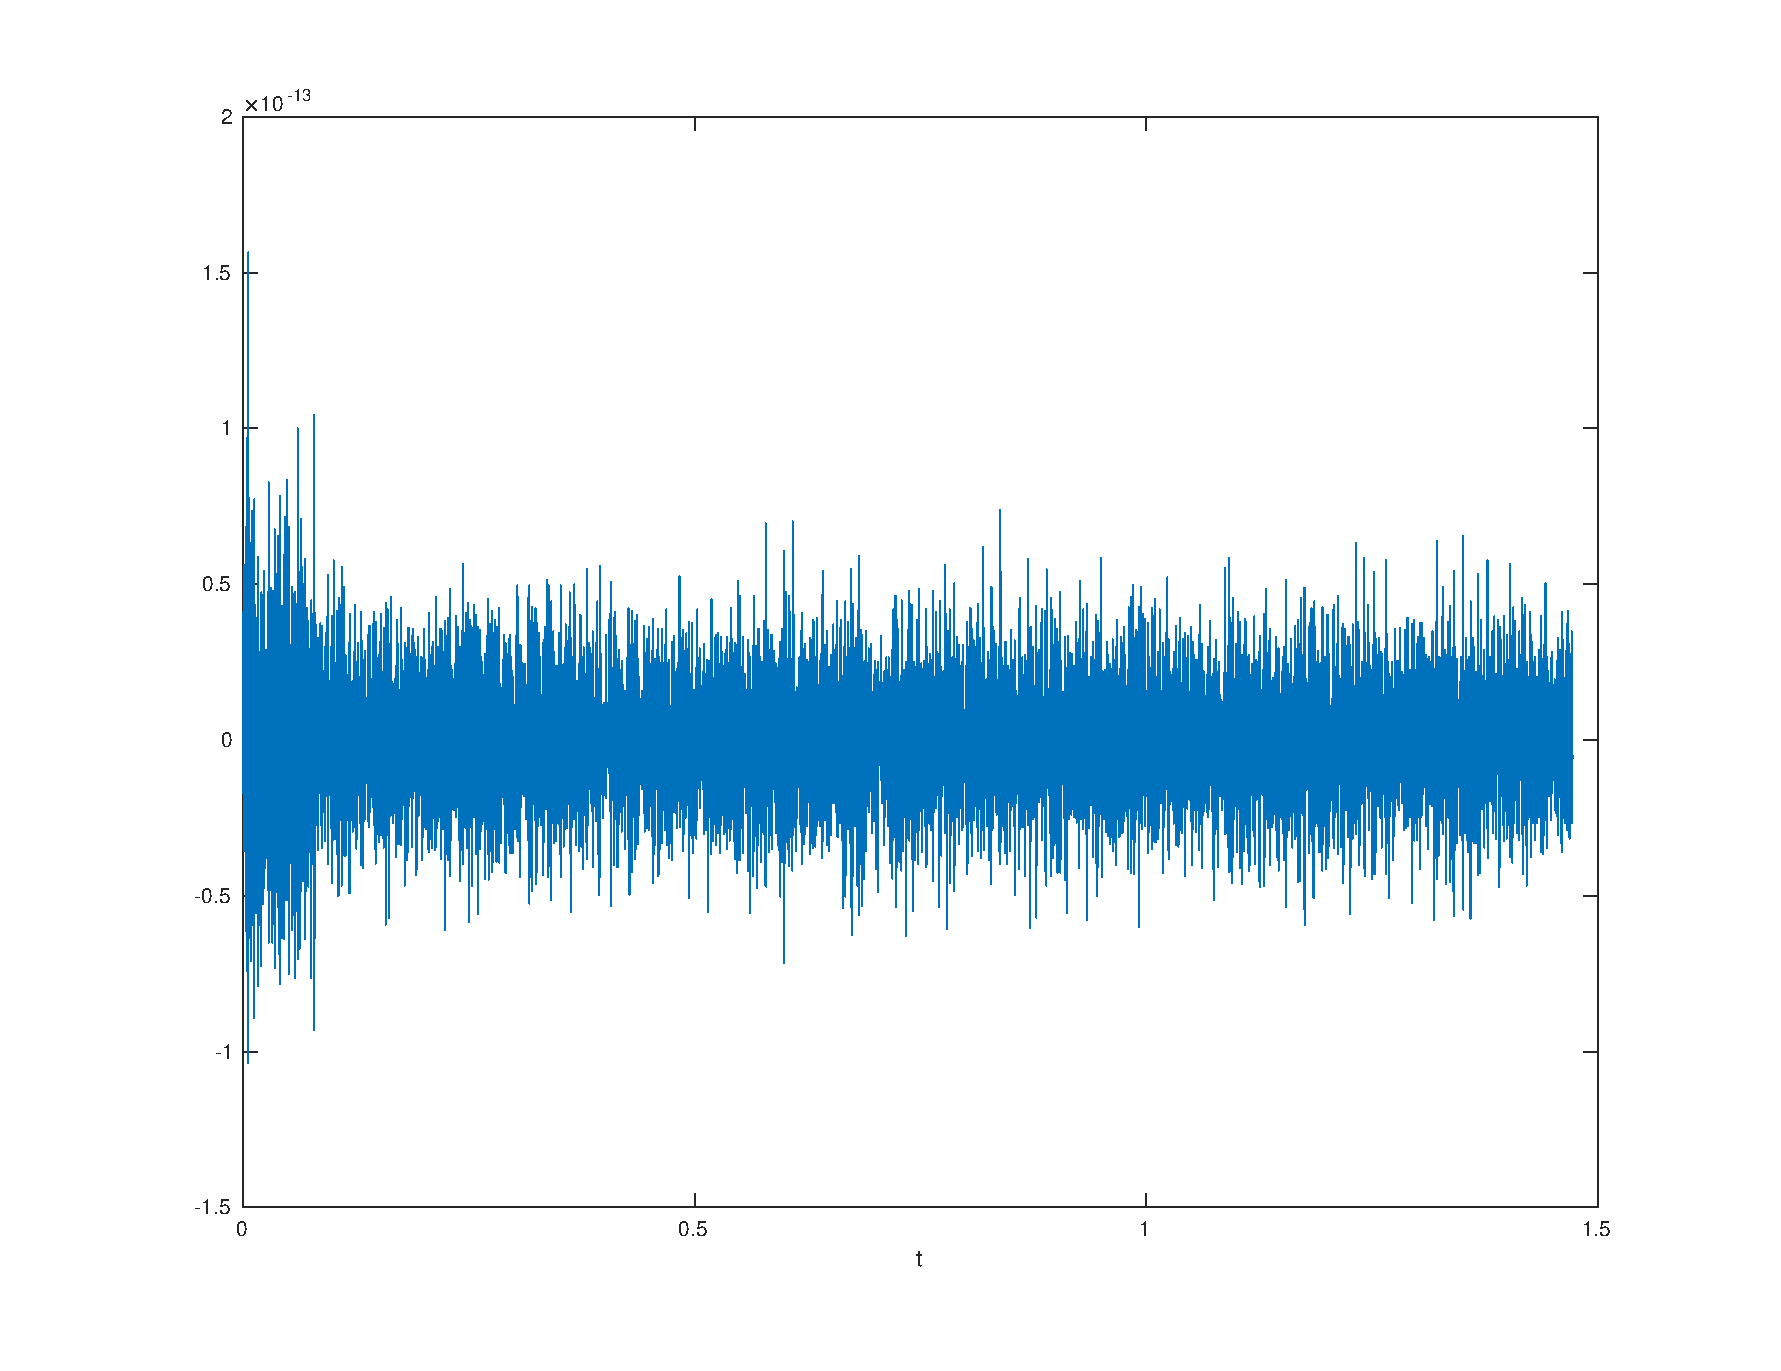
\includegraphics[width=\textwidth]{images/cons_mass.eps}\hfill
        \caption{Energy}
        \label{fig:Energy}
    \end{subfigure}
    \hfill
    \begin{subfigure}[b]{0.45\textwidth}
        \centering
        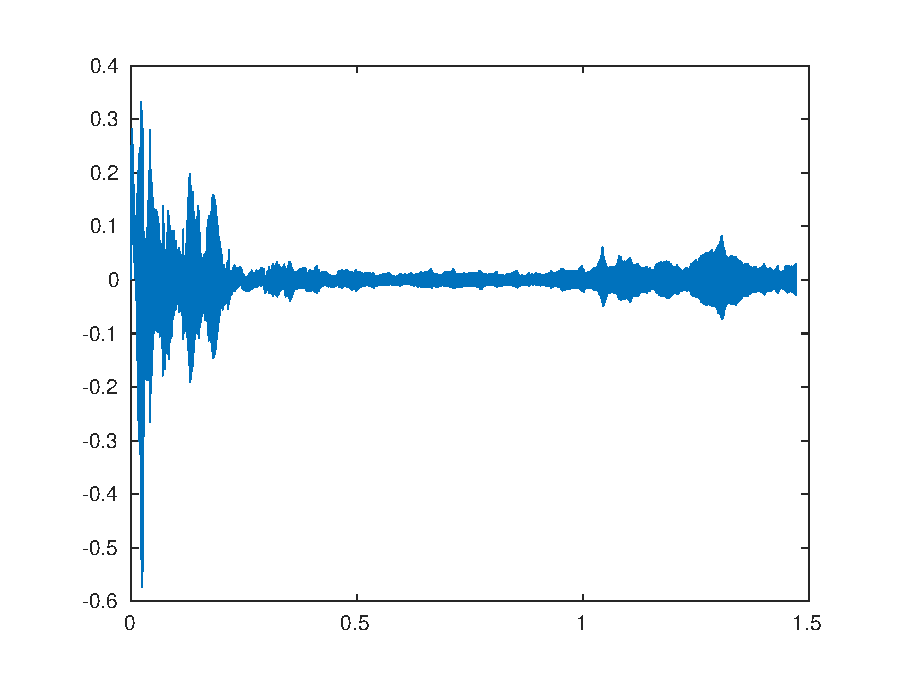
\includegraphics[width=\textwidth]{images/cons_energy.eps}\hfill
        \caption{Mass}
        \label{fig:Mass}
    \end{subfigure}
    \caption{2d conservation plots for mass, and energy.}
    \label{fig:three graphs}
\end{figure}

\begin{figure}[htp]
    \centering
    \begin{subfigure}[b]{0.3\textwidth}
        \centering
        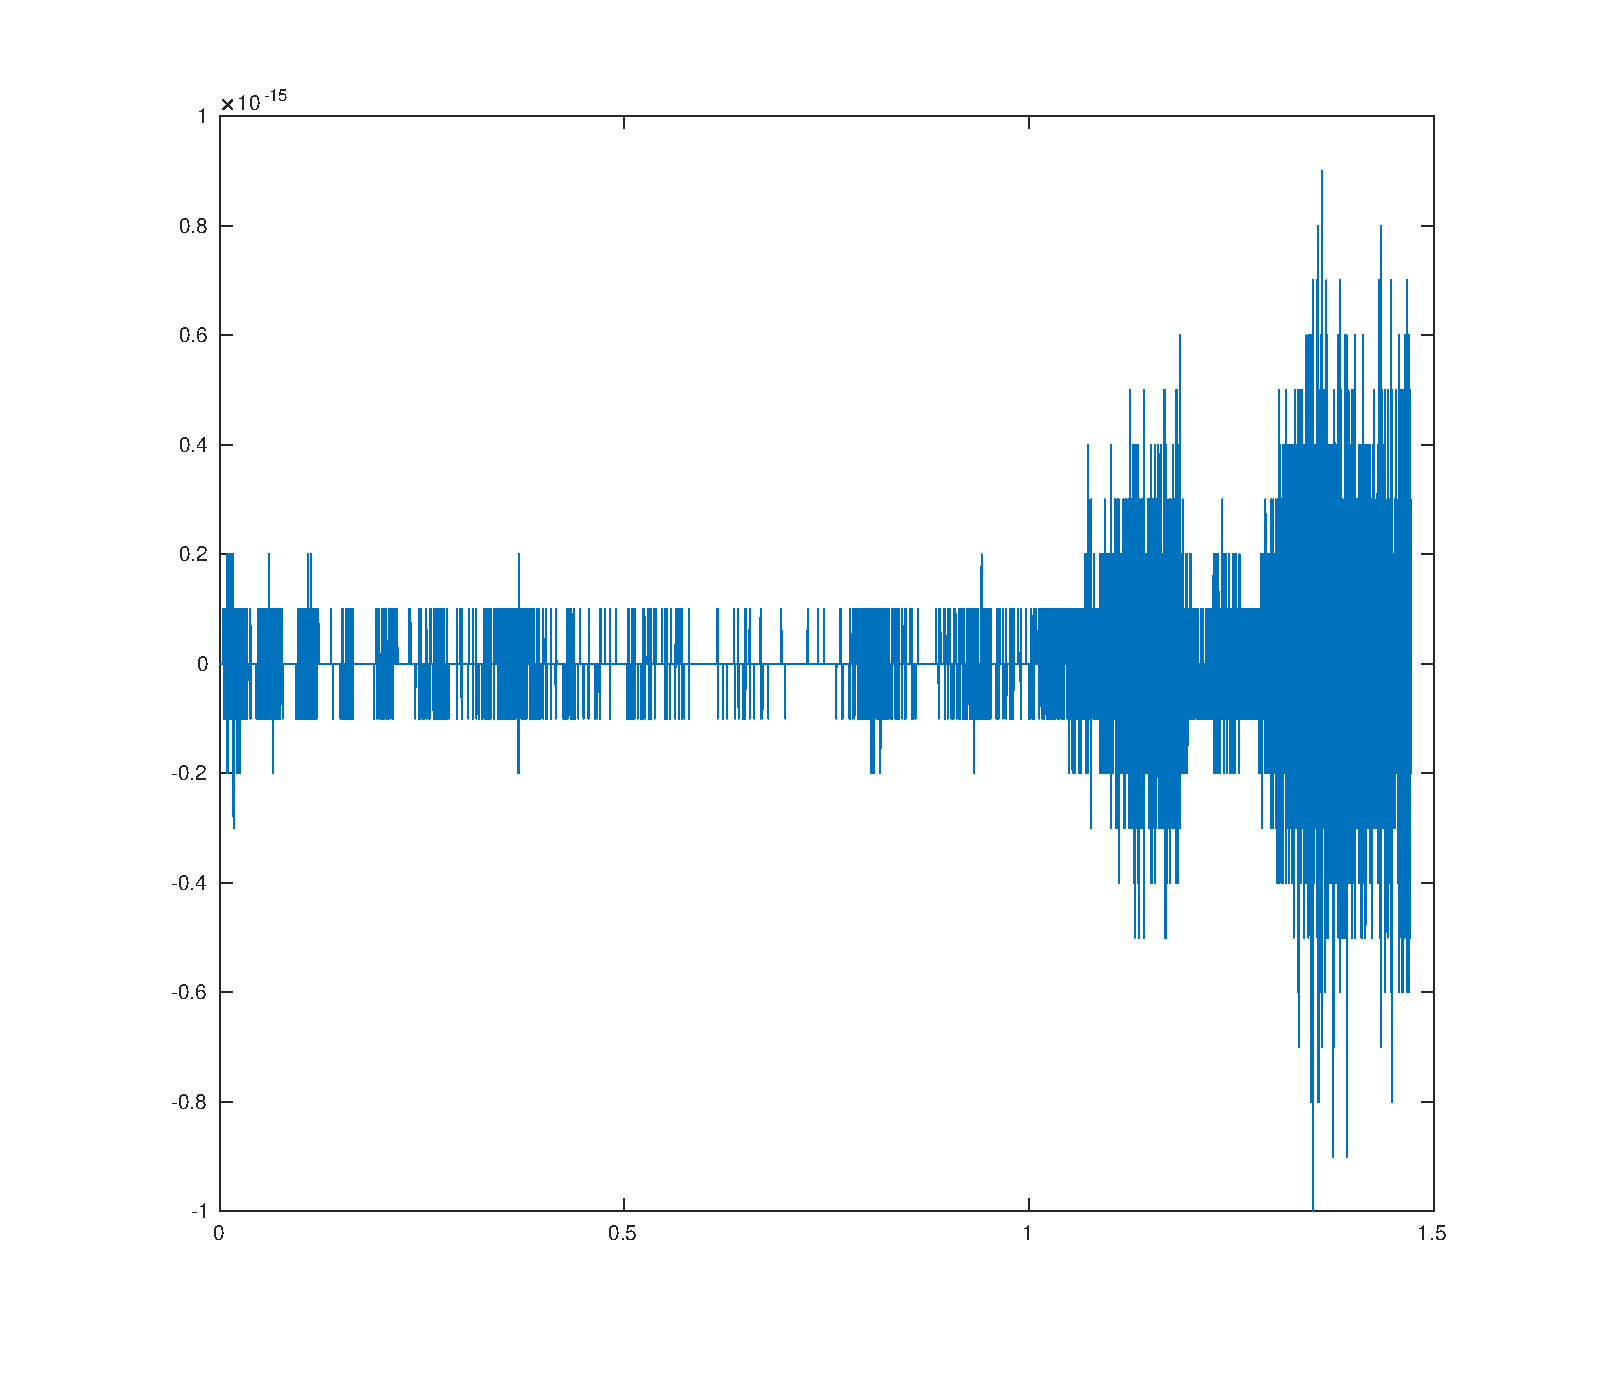
\includegraphics[width=\textwidth]{images/cons_momu.eps}\hfill
        \caption{u-momentum}
        \label{fig:Energy}
    \end{subfigure}
    \hfill
    \begin{subfigure}[b]{0.3\textwidth}
        \centering
        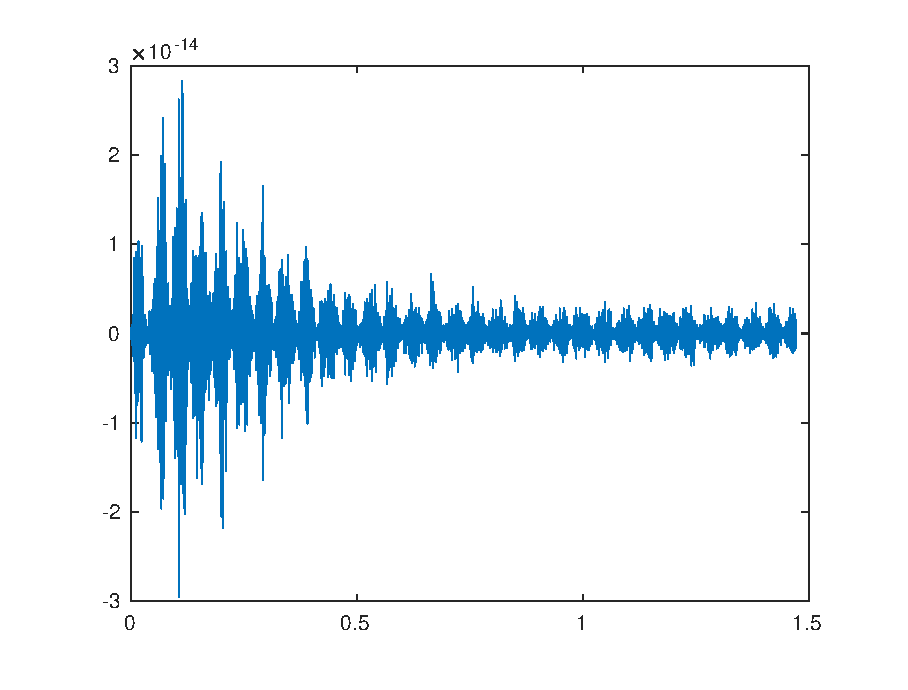
\includegraphics[width=\textwidth]{images/cons_momv.eps}\hfill
        \caption{v-momentum}
        \label{fig:Mass}
    \end{subfigure}
    \hfill
    \begin{subfigure}[b]{0.3\textwidth}
        \centering
        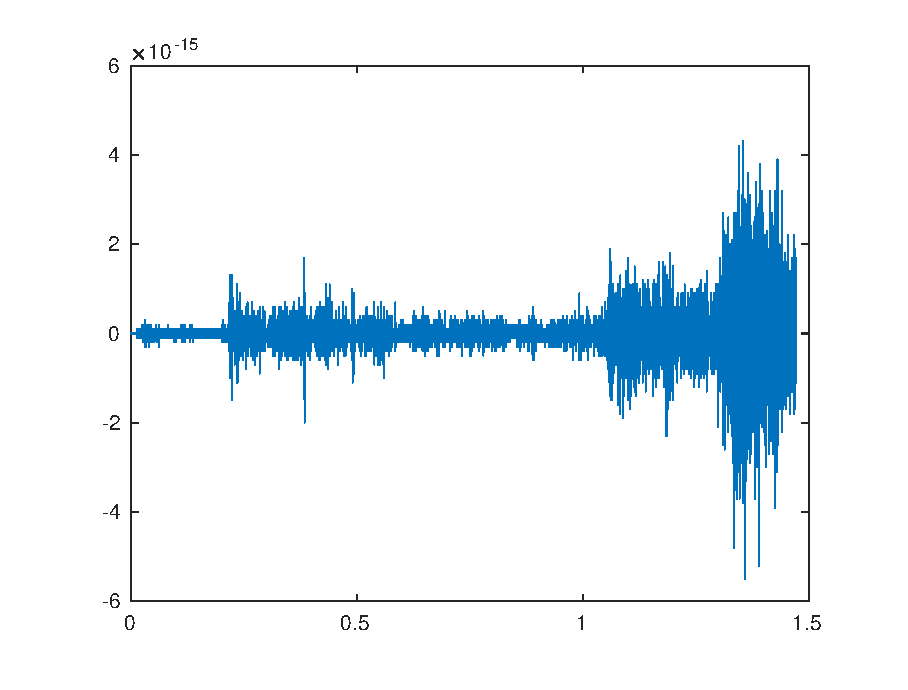
\includegraphics[width=\textwidth]{images/cons_vort.eps}\hfill
        \caption{vorticity}
        \label{Momentum}
    \end{subfigure}
     \hfill
    \caption{2D Conservation plots.}
    \label{fig:three graphs}
\end{figure}



Lorem ipsum dolor sit amet, ad vix saperet mediocrem consetetur, ut admodum torquatos maiestatis est, 
no aeque singulis interpretaris sea. Ut paulo petentium eum, eum id malorum dignissim. Sed ex modus quodsi. 
Simul commodo scribentur ne has, mei ei dico interpretaris. Iriure tibique gloriatur vim an. Mea ea idque 
fabulas lucilius.

Vel timeam fuisset te. Duo ea nobis omnium pericula, sed discere scripserit ei, mea an illud dolore adolescens.
 Eu cum eligendi voluptatum, brute lobortis eam an, ea mei fastidii complectitur. An causae accusam pri. 
 In ius possit oportere.ges: